% ============================================================
% Chapter 5: Hilbert's Problem 4 — The Shortest Path as the Straight Line
% ============================================================

\chapter{The Shortest Path Between Two Points}

\begin{solvedbox}
Hilbert's Fourth Problem asks whether the straight line is always the shortest path between two points, and more broadly, what foundations are needed to make rigorous the notion of ``distance'' in geometry. The problem is resolved: the development of metric spaces, Riemannian geometry, and Finsler geometry provides a complete and flexible framework in which the question of shortest paths---and the role of straight lines---is fully understood.
\end{solvedbox}

\section{Historical Context}

The idea that a straight line is the shortest path between two points is so ancient and so intuitive that it barely seems like a claim at all. Euclid stated it as a common notion in the \emph{Elements} (circa 300~BCE): ``Of all lines which join a point to a line, the perpendicular is the shortest.'' His axioms treat the straight line as self-evidently the most direct connection between two locations.

For over two thousand years, this idea went largely unquestioned---not because mathematicians were lazy, but because Euclid's framework was so natural. The \emph{straight line} was \emph{defined}, in effect, by its directness. The \emph{distance} between two points was the length of the straight segment joining them.

By the 19th century, however, cracks had appeared. Non-Euclidean geometries showed that parallel lines need not behave as Euclid assumed. Riemann's 1854 dissertation showed that geometry could be studied on curved surfaces---surfaces where the ``straight line'' might not even exist in the Euclidean sense. On a sphere, for example, the shortest path between two points is a great circle arc, not a Euclidean line.

These developments raised a fundamental question: What does it \emph{mean} for a path to be the ``shortest''? What does it mean for a space to have a notion of ``distance''? And is the straight line---in some generalized sense---always the shortest path?

Hilbert himself had already grappled with these questions in his 1899 masterpiece \emph{Grundlagen der Geometrie} (``Foundations of Geometry''), where he gave the first complete axiomatic treatment of Euclidean geometry. Problem~4 asks us to extend this axiomatic clarity to the very concept of distance itself.

\section{The Problem}

Hilbert's Fourth Problem can be stated informally:

\begin{problem_statement}
Is the straight line the shortest connection between two points? More precisely, can we axiomatize geometry so that the straight line is always characterized as the shortest path, and what are the proper foundations for the concept of distance?
\end{problem_statement}

To make this question precise, we need to address three sub-questions:
\begin{enumerate}
    \item \textbf{What is a ``distance''?} We need a rigorous definition of the distance between two points that goes beyond the Euclidean case.
    \item \textbf{What is a ``shortest path''?} Given a notion of distance, we need to define what it means for a curve to minimize distance between two points.
    \item \textbf{When is the shortest path a ``straight line''?} We need to understand the relationship between the metric structure of a space and the geodesics---the curves that play the role of straight lines.
\end{enumerate}
The resolution of these questions led to some of the significant developments in modern geometry.

\section{Key Developments}

\subsection{Metric Spaces: The Abstract Notion of Distance}

The first step was to abstract the notion of distance. In 1906---just six years after Hilbert's lecture---Maurice Fr\'echet introduced the concept of a \emph{metric space}, providing a rigorous foundation for the idea of distance.

\begin{definition}
A \textbf{metric space} is a set $X$ together with a function $d : X \times X \to \mathbb{R}$ (called a \textbf{metric}) satisfying, for all $x, y, z \in X$:
\begin{enumerate}
    \item \textbf{Non-negativity:} $d(x,y) \geq 0$, with $d(x,y) = 0$ if and only if $x = y$.
    \item \textbf{Symmetry:} $d(x,y) = d(y,x)$.
    \item \textbf{Triangle inequality:} $d(x,z) \leq d(x,y) + d(y,z)$.
\end{enumerate}
\end{definition}

The triangle inequality is the key axiom: it captures the idea that going directly from $x$ to $z$ is never worse than going through an intermediate point $y$. This is the abstract essence of ``the straight line is the shortest path.''

In $\mathbb{R}^n$, the familiar Euclidean metric
\[
    d(x,y) = \sqrt{(x_1 - y_1)^2 + (x_2 - y_2)^2 + \cdots + (x_n - y_n)^2}
\]
is the most natural choice, but it is far from the only one. Consider, for example, the \emph{taxicab metric} on $\mathbb{R}^2$:
\[
    d_1(x,y) = |x_1 - y_1| + |x_2 - y_2|.
\]
This satisfies all the axioms of a metric, but in this metric, the ``shortest path'' from $(0,0)$ to $(1,1)$ is not unique---any monotone staircase path has the same length. The geometry of the space depends crucially on which metric we choose.

\begin{example}[Non-unique geodesics in the taxicab metric]
In the Euclidean metric, the unique shortest path from $(0,0)$ to $(1,1)$ is the straight-line segment. In the taxicab metric $d_1$, the distance is $2$, and \emph{any} path that moves only right and up (never backtracking) has length exactly $2$:
\[
\begin{array}{lll}
\text{Path A:} & (0,0) \to (1,0) \to (1,1) & \text{(right, then up)} \\
\text{Path B:} & (0,0) \to (0,1) \to (1,1) & \text{(up, then right)} \\
\text{Path C:} & (0,0) \to (0.5,0) \to (0.5,1) \to (1,1) & \text{(zigzag)}
\end{array}
\]
Any path composed of axis-aligned segments that never backtracks has total length $|x_1-x_2|+|y_1-y_2|$ in this metric. The straight diagonal line also has length $2$---the same as the staircase paths---so the shortest path is far from unique. This shows that Hilbert's question ``is the straight line the shortest path?'' cannot be answered without first specifying the metric.
\end{example}

\begin{figure}[htbp]
\centering
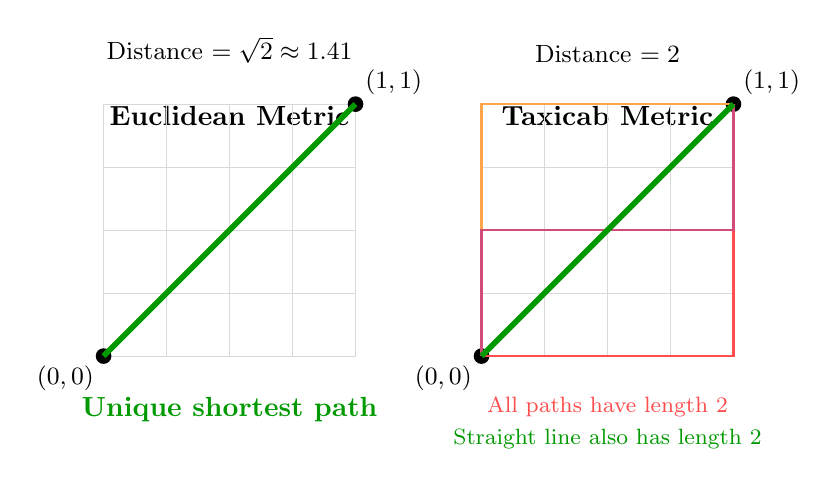
\begin{tikzpicture}[
    scale=0.8,
    font=\small,
    grid/.style={help lines, color=gray!30},
    point/.style={circle, fill=black, inner sep=2pt},
    path/.style={thick, color=blue!70}
]

% Euclidean metric (left)
\node[above, font=\bfseries] at (2, 3.5) {\textbf{Euclidean Metric}};

% Grid
\draw[grid] (0,0) grid (4,4);

% Start and end points
\node[point] at (0,0) {};
\node[point] at (4,4) {};
\node[below left] at (0,0) {$(0,0)$};
\node[above right] at (4,4) {$(1,1)$};

% Unique shortest path (straight line)
\draw[path, color=green!60!black, line width=2pt] (0,0) -- (4,4);

% Label
\node[below, color=green!60!black, font=\bfseries] at (2, -0.5) {Unique shortest path};

% Taxicab metric (right)
\node[above, font=\bfseries] at (8, 3.5) {\textbf{Taxicab Metric}};

% Grid
\draw[grid] (6,0) grid (10,4);

% Start and end points
\node[point] at (6,0) {};
\node[point] at (10,4) {};
\node[below left] at (6,0) {$(0,0)$};
\node[above right] at (10,4) {$(1,1)$};

% Multiple shortest paths
\draw[path, color=red!70] (6,0) -- (10,0) -- (10,4);
\draw[path, color=orange!70] (6,0) -- (6,4) -- (10,4);
\draw[path, color=purple!70] (6,0) -- (6,2) -- (10,2) -- (10,4);

% Straight line (same length!)
\draw[path, color=green!60!black, line width=2pt] (6,0) -- (10,4);

% Labels
\node[below, color=red!70, font=\footnotesize] at (8, -0.5) {All paths have length $2$};
\node[below, color=green!60!black, font=\footnotesize] at (8, -1.0) {Straight line also has length $2$};

% Distance annotations
\node[above, font=\small] at (2, 4.5) {Distance $= \sqrt{2} \approx 1.41$};
\node[above, font=\small] at (8, 4.5) {Distance $= 2$};

\end{tikzpicture}
\caption{Comparison of shortest paths in Euclidean and taxicab metrics. In the Euclidean metric (left), the straight line is the unique shortest path. In the taxicab metric (right), infinitely many staircase paths achieve the same minimal length as the straight line.}
\label{fig:taxicab}
\end{figure}

\subsection{Riemannian Geometry: Distance on Curved Spaces}

The deeper question is: how do we define distance on a curved surface or manifold? Bernhard Riemann answered this in his 1854 \emph{Habilitationsschrift}, laying the foundation for what is now called \textbf{Riemannian geometry}.

A Riemannian manifold is a smooth manifold $M$ equipped with a \emph{Riemannian metric} $g$---a smoothly varying inner product on the tangent space at each point. Intuitively, $g$ tells us how to measure lengths of tangent vectors at every point of the manifold.

Given a smooth curve $\gamma : [a,b] \to M$, its \textbf{length} is defined by
\[
    L(\gamma) = \int_a^b \sqrt{g_{\gamma(t)}(\dot\gamma(t), \dot\gamma(t))} \, dt.
\]
The \textbf{distance} between two points $p, q \in M$ is then the infimum of the lengths of all smooth curves connecting $p$ to $q$:
\[
    d(p,q) = \inf_{\gamma} L(\gamma).
\]
This gives a well-defined metric on $M$ (at least when $M$ is connected), and it generalizes the Euclidean notion of distance to curved spaces.

\subsubsection*{Geodesics}

A curve achieving the infimum---one of locally minimal length---is called a \textbf{geodesic}. Geodesics play the role of ``straight lines'' in Riemannian geometry. They are determined by the geodesic equation:
\[
    \ddot{x}^k + \sum_{i,j} \Gamma^k_{ij} \, \dot{x}^i \, \dot{x}^j = 0,
\]
where the $\Gamma^k_{ij}$ are the Christoffel symbols derived from the metric $g$. In flat Euclidean space, geodesics are ordinary straight lines. But on curved surfaces, geodesics can behave quite differently.

\subsubsection*{Examples of Geodesics}

\begin{itemize}
    \item \textbf{Euclidean geometry} ($\mathbb{R}^n$ with the standard metric): Geodesics are straight lines. This is the classical case where the straight line really is the shortest path.

    \item \textbf{Spherical geometry} (the surface $S^2$ of a sphere with the metric induced from $\mathbb{R}^3$): Geodesics are \emph{great circles}---circles whose center is the center of the sphere. The shortest path from New York to London is not a ``straight line'' drawn on a flat map, but a great circle arc on the globe. Pilots and sailors have known this empirically for centuries.

    \item \textbf{Hyperbolic geometry} (the hyperbolic plane $\mathbb{H}^2$ with its constant negative curvature): Geodesics are arcs of circles perpendicular to the boundary of the Poincar\'e disk model (or semicircles centered on the real axis in the upper half-plane model). Here, parallel geodesics \emph{diverge} rather than remaining equidistant, a clear departure from Euclidean intuition.
\end{itemize}
These three examples---Euclidean, spherical, and hyperbolic---represent the three types of constant-curvature geometry, and they illustrate how different the ``shortest path'' can look depending on the underlying metric.

\subsubsection*{Worked Example: Geodesics on a Sphere via the Euler--Lagrange Equation}

Let us derive the geodesics on a sphere of radius $R$ using the calculus of variations. In spherical coordinates $(\theta,\phi)$, where $\theta\in[0,\pi]$ is the polar angle and $\phi\in[0,2\pi)$ the azimuthal angle, the metric is
\[
ds^2 = R^2\,d\theta^2 + R^2\sin^2\theta\,d\phi^2.
\]

For a curve $\gamma(t)=(\theta(t),\phi(t))$ with $t\in[a,b]$, the length functional is
\[
L[\gamma] = R\int_a^b\sqrt{\dot\theta^2 + \sin^2\theta\,\dot\phi^2}\;dt.
\]

The integrand $F = \sqrt{\dot\theta^2 + \sin^2\theta\,\dot\phi^2}$ does not depend on $\phi$ explicitly, so the Euler--Lagrange equation for $\phi$ gives a first integral:
\[
\frac{\partial F}{\partial\dot\phi}
= \frac{\sin^2\theta\,\dot\phi}{\sqrt{\dot\theta^2 + \sin^2\theta\,\dot\phi^2}}
= \text{constant}.
\]

Parametrizing by arc length $s$ sets the denominator to $1$ (since $\|\gamma'(s)\|=1$), yielding
\[
\sin^2\theta\,\phi' = C,
\tag{1}
\]
where $'=d/ds$ and $C$ is a constant---a conserved angular momentum component.

The Euler--Lagrange equation for $\theta$ gives
\[
\frac{d}{ds}\!\left(\frac{\partial F}{\partial\theta'}\right) = \frac{\partial F}{\partial\theta}
\;\Longrightarrow\;
\theta'' = \sin\theta\cos\theta\,(\phi')^2.
\tag{2}
\]

Now we check that great circles satisfy (1) and~(2).

\paragraph{Meridians ($\phi = \text{constant}$).}
Here $\phi' = 0$, so (1) holds with $C=0$. Equation~(2) becomes $\theta'' = 0$, so $\theta$ is linear in $s$. The curve is a great circle through the poles---a line of constant longitude.

\paragraph{The equator ($\theta = \pi/2$).}
Then $\theta' = 0$, $\theta'' = 0$, $\sin\theta = 1$, and $\cos\theta = 0$. Equation~(2) gives $0 = 0$, and (1) gives $\phi' = C$, which is constant. The equator is therefore a geodesic.

By the rotational symmetry of the sphere, \emph{every} great circle can be rotated to the equator or to a meridian. Since the geodesic equations are preserved under rotations, all great circles are geodesics. This is why the shortest path between two cities is a great-circle arc.

\subsubsection*{Worked Example: Geodesics in the Poincar\'e Upper Half-Plane}

The Poincar\'e upper half-plane is $\mathbb{H} = \{x + iy \mid y > 0\}$ with the metric
\[
ds^2 = \frac{dx^2 + dy^2}{y^2}.
\]

For a curve $(x(t),y(t))$ the length functional is $L = \int \sqrt{\dot x^2 + \dot y^2}\,y^{-1}\,dt$. The integrand $F = \sqrt{\dot x^2 + \dot y^2}/y$ does not depend on $x$, giving the first integral
\[
\frac{\partial F}{\partial\dot x}
= \frac{\dot x}{y\sqrt{\dot x^2 + \dot y^2}}
= \text{constant}.
\]

Parametrizing by arc length $s$ sets $\sqrt{x'^2 + y'^2}/y = 1$, so the conserved quantity simplifies to
\[
\frac{x'}{y^2} = k \quad\Longrightarrow\quad x' = k\,y^2.
\tag{3}
\]

The arc-length condition gives $x'^2 + y'^2 = y^2$. Substituting (3):
\[
k^2 y^4 + y'^2 = y^2 \quad\Longrightarrow\quad y'^2 = y^2(1 - k^2 y^2).
\tag{4}
\]

Dividing (3) by (4):
\[
\frac{dy}{dx} = \frac{y'}{x'} = \frac{\pm y\sqrt{1 - k^2 y^2}}{k y^2}
= \pm \frac{\sqrt{1 - k^2 y^2}}{k y},
\qquad
\frac{dx}{dy} = \pm \frac{k y}{\sqrt{1 - k^2 y^2}}.
\]

Integrating: $x(y) = C \mp \frac{1}{k}\sqrt{1 - k^2 y^2}$, which rearranges to
\[
(x - C)^2 + y^2 = \frac{1}{k^2}.
\tag{5}
\]

This is the equation of a circle with center $(C,0)$ on the real axis and radius $1/|k|$. Since $y > 0$ in $\mathbb{H}$, only the upper semicircle lies in the half-plane.

\begin{example}[Geodesics in $\mathbb{H}$, continued]
Geodesics in the Poincar\'e upper half-plane are of two types:
\begin{itemize}
    \item \textbf{Vertical lines} ($x = \text{constant}$), obtained when $k = 0$ in~(3). These can be thought of as semicircles of infinite radius.
    \item \textbf{Semicircles centered on the real axis}, given by equation~(5).
\end{itemize}
Both types are orthogonal to the boundary $y = 0$ (the real axis). This is the hyperbolic analogue of straight lines: the ``shortest path'' is a semicircular arc, not a Euclidean straight line.
\end{example}

\subsection{Hilbert's Axiomatic Approach: The Grundlagen der Geometrie}

Hilbert did not merely pose Problem~4---he had already laid the groundwork for its resolution. In 1899, one year before his Paris lecture, Hilbert published \emph{Grundlagen der Geometrie} (``Foundations of Geometry''), a landmark work that gave the first complete, rigorous axiomatization of Euclidean geometry.

The \emph{Grundlagen} identifies five groups of axioms: incidence, order, congruence, parallels, and continuity. In this framework, the straight line is not defined by its minimal-length property; rather, it is a primitive notion governed by the incidence and order axioms. The statement ``the straight line is the shortest path between two points'' becomes a \emph{theorem} (the triangle inequality) that follows from the axioms, not a definition.

This separation---between the axiomatic definition of ``straight line'' and the metric notion of ``shortest path''---was a significant conceptual advance. Hilbert showed that the Euclidean straight line could be characterized either by its geometric axioms (determined by two points, extends infinitely, etc.) or by its metric property (minimizes distance). Problem~4 asks essentially: \emph{are these two characterizations always the same?} The answer depends on the geometry. In Riemannian geometry, geodesics generalize both roles; in Finsler geometry, they retain the metric role but may look very different from Euclidean lines.

\subsection{Finsler Geometry: A Further Generalization}

Riemannian geometry measures lengths using an inner product on tangent spaces. Paul Finsler, in his 1918 thesis, generalized this further. A \textbf{Finsler metric} replaces the inner product with a more general \emph{norm} on each tangent space.

\begin{definition}
A \textbf{Finsler metric} on a manifold $M$ is a function $F : TM \to [0,\infty)$ (where $TM$ is the tangent bundle) satisfying:
\begin{enumerate}
    \item \textbf{Positive homogeneity:} $F(\lambda v) = |\lambda| \, F(v)$ for all $\lambda \in \mathbb{R}$ and tangent vectors $v$.
    \item \textbf{Strong convexity:} The function $v \mapsto F(v)^2$ is smooth and its Hessian is positive definite away from the zero section.
\end{enumerate}
\end{definition}

Every Riemannian metric is a Finsler metric (take $F(v) = \sqrt{g(v,v)}$), but Finsler metrics are more general. A simple example is the \emph{taxicab norm} on $\mathbb{R}^2$: $F(v) = |v_1| + |v_2|$. In Finsler geometry, the shortest path depends not only on where you are but also on the direction you are traveling. This makes Finsler geometry natural for modeling anisotropic media.

The geodesic equation also generalizes. In Riemannian geometry the Christoffel symbols depend only on position; in Finsler geometry they depend on velocity as well. The Finsler geodesic equation is
\[
\ddot{x}^i + 2 G^i(x,\dot{x}) = 0,
\]
where $G^i$ are the \emph{geodesic spray coefficients}
\[
G^i(x,y) = \frac{1}{4}\, g^{i\ell}(x,y)\left(
\frac{\partial^2 F^2}{\partial x^k\,\partial y^\ell}\,y^k - \frac{\partial F^2}{\partial x^\ell}
\right),
\]
with $g_{ij}(x,y) = \frac12\frac{\partial^2 F^2}{\partial y^i\,\partial y^j}$ the Finsler metric tensor (now direction-dependent). When $F$ comes from a Riemannian metric, $g_{ij}$ is independent of $y$ and $2G^i$ reduces to $\Gamma^i_{jk}(x)\,y^j y^k$.

Finsler geometry provides the most general framework in which Hilbert's question can be posed. The answer: it depends on the metric. Geodesics are well-defined curves of minimal length, but they may or may not be ``straight'' in any conventional sense.

\subsection{The Role of Hilbert's Problem}

Hilbert's Fourth Problem was, in a sense, a question about foundations: what is the right framework for discussing ``distance'' and ``shortest path''? The answer came not from a single theorem, but from the gradual development of a rich mathematical landscape:
\begin{itemize}
    \item Fr\'echet's metric spaces provided the abstract framework.
    \item Riemannian geometry provided the tools for studying distance on curved spaces.
    \item Finsler geometry generalized Riemannian geometry to the most flexible setting.
    \item The theory of geodesics unified the concept of ``straight line'' across all these settings.
\end{itemize}
Hilbert's question was not so much a problem to be ``solved'' as a direction to be explored---and the exploration led to some of the significant geometry of the 20th century.

\section{Why This Matters: Geodesics in Physics}

The mathematics of shortest paths is not merely abstract. In 1915, Albert Einstein formulated his general theory of relativity, which describes gravity as the curvature of spacetime. In this theory, massive objects curve the four-dimensional spacetime manifold, and freely falling particles move along \emph{timelike geodesics} of this curved spacetime.

The geodesic equation in general relativity is formally identical to the one in Riemannian geometry:
\[
\frac{d^2 x^\mu}{d\tau^2} + \Gamma^\mu_{\nu\rho}\,\frac{dx^\nu}{d\tau}\frac{dx^\rho}{d\tau} = 0,
\]
where $\tau$ is proper time along the particle's worldline and the Christoffel symbols $\Gamma^\mu_{\nu\rho}$ are computed from the spacetime metric $g_{\mu\nu}$, which satisfies Einstein's field equations.

\begin{example}[Light deflection by the Sun]
One of the classic tests of general relativity is the bending of starlight by the Sun's gravitational field. Light follows \emph{null geodesics} ($ds^2 = 0$) through curved spacetime. Near the Sun, the spacetime metric is approximately the Schwarzschild metric
\[
ds^2 = -\left(1-\frac{2GM}{rc^2}\right)c^2 dt^2 + \left(1-\frac{2GM}{rc^2}\right)^{-1}dr^2 + r^2(d\theta^2 + \sin^2\theta\,d\phi^2).
\]
Solving the null geodesic equation for a light ray passing near the Sun predicts a deflection angle of about $1.75$ arcseconds---a prediction famously confirmed by Eddington's 1919 solar eclipse expedition. The ``straight line'' in curved spacetime is a geodesic of the Riemannian geometry of spacetime, not a Euclidean straight line.
\end{example}

Thus Hilbert's fourth problem---the question of what it means for a path to be the shortest---is deeply connected to our understanding of the physical universe. The geometry of shortest paths is the geometry of gravity itself.

\section{Current Status}

\begin{solvedbox}
Hilbert's Fourth Problem is resolved. The proper foundations for the concept of distance---metric spaces, Riemannian geometry, and Finsler geometry---are well established. The question of when the ``straight line'' is the shortest path is fully understood: it is a property of the metric, not an absolute truth. The development of these frameworks constitutes a complete answer to the foundational question Hilbert posed.
\end{solvedbox}

\section*{Common Questions}

\begin{description}[font=\bfseries, leftmargin=2em, style=nextline]

\item[Q: If a geodesic is the shortest path, how can there be multiple geodesics between two points?]\hfill\\
The defining property of a geodesic is that it is \emph{locally} shortest: any small segment is the shortest path between its endpoints. A geodesic need not be globally shortest. On a sphere, for example, there are two great-circle arcs between most pairs of points (the short one and the long one), and both are geodesics. The long one is still locally shortest even though it is not the global shortest path. On a cylinder, you can have infinitely many geodesics between two points that wrap around different numbers of times.

\item[Q: Is Hilbert's problem really about geometry or about defining distance?]\hfill\\
Both. Hilbert's fourth problem asks to characterize all metrics whose geodesics are straight lines---a question about the relationship between distance and the structure of space. This sits at the intersection of geometry (what shapes are possible?), analysis (what counts as a metric?), and foundations (how should we define distance in the first place?).

\item[Q: What's the difference between a metric and a Riemannian metric?]\hfill\\
A \emph{metric} (in the sense of metric spaces) is a distance function $d(x,y)$ satisfying symmetry, positivity, and the triangle inequality. A \emph{Riemannian metric} is a smoothly varying inner product on the tangent spaces of a manifold, from which one can define lengths of curves and then a distance function by taking the infimum of curve lengths. Every Riemannian manifold is a metric space, but not every metric space comes from a Riemannian metric---the taxicab metric on $\mathbb{R}^2$, for example, is not Riemannian because it does not arise from a smooth inner product.

\item[Q: Do shortest paths always exist in a metric space?]\hfill\\
No. The Hopf--Rinow theorem guarantees that geodesics exist between any two points in a complete Riemannian manifold. But in a general metric space, a shortest path may not exist---there might be a sequence of paths whose lengths approach the distance but no path actually achieving it. For example, in the punctured plane $\mathbb{R}^2 \setminus \{0\}$, there is no shortest path between two points on opposite sides of the origin if the straight line would pass through the missing point.

\item[Q: How does the Euler--Lagrange equation relate to geodesics?]\hfill\\
Finding the shortest path between two points is a calculus of variations problem: minimize the length functional $L[\gamma] = \int |\gamma'(t)| \, dt$. A geodesic is a critical point of this functional, just as a minimum of a function $f(x)$ occurs at a critical point where $f'(x)=0$. The Euler--Lagrange equation gives the necessary condition: it yields the geodesic equation $\nabla_{\gamma'}\gamma' = 0$, which says the curve has zero acceleration in the geometry defined by the metric.

\item[Q: Are geodesics always unique?]\hfill\\
No. On a sphere, two antipodal points are connected by infinitely many great-circle geodesics (all great circles through both poles). On a cylinder, two points can be connected by geodesics that wind around different numbers of times. In a flat torus, there are infinitely many geodesics between any two points. Uniqueness of geodesics is a special property of certain spaces (like Euclidean space or hyperbolic space with no conjugate points), not a general property.

\end{description}

\section{Exercises}

\begin{enumerate}

    \item \textbf{Different metrics on $\mathbb{R}^2$.} Consider the following three metrics on $\mathbb{R}^2$:
    \begin{itemize}
        \item The Euclidean metric: $d_E(x,y) = \sqrt{(x_1-y_1)^2 + (x_2-y_2)^2}$.
        \item The taxicab metric: $d_1(x,y) = |x_1-y_1| + |x_2-y_2|$.
        \item The supremum metric: $d_\infty(x,y) = \max\{|x_1-y_1|, |x_2-y_2|\}$.
    \end{itemize}
    Verify that each of these is indeed a metric. Draw the ``unit circle'' $\{x : d(x, 0) = 1\}$ for each. How do the shapes differ?

    \item \textbf{Geodesics on the sphere.} The sphere $S^2$ of radius $R$ can be parametrized by spherical coordinates $(\theta, \phi)$ where $\theta \in [0, \pi]$ is the polar angle and $\phi \in [0, 2\pi)$ is the azimuthal angle. The metric is
    \[
        ds^2 = R^2 \, d\theta^2 + R^2 \sin^2\theta \, d\phi^2.
    \]
    \begin{enumerate}
        \item Compute the length of a great circle arc from the north pole $(\theta = 0)$ to a point at polar angle $\theta_0$. Verify that it equals $R\theta_0$.
        \item Two cities are at the same latitude $\theta_0$ but differ in longitude by $\Delta\phi$. Is the great circle path between them also at latitude $\theta_0$? (Hint: think about flights from New York to Madrid.)
    \end{enumerate}

    \item \textbf{The taxicab geometry.} In the taxicab metric $d_1$ on $\mathbb{R}^2$, describe all shortest paths from $(0,0)$ to $(3,2)$. What do they look like geometrically?

    \item \textbf{A non-Euclidean metric.} Define a metric on the open interval $(0, \infty)$ by
    \[
        d(x,y) = \left|\frac{1}{x} - \frac{1}{y}\right|.
    \]
    \begin{enumerate}
        \item Verify the three metric axioms.
        \item Is this metric complete? (A metric space is \emph{complete} if every Cauchy sequence converges.)
        \item Can you find a bijection from $((0,\infty), d)$ to $(\mathbb{R}, d_E)$ that is an isometry?
    \end{enumerate}

    \item \textbf{Geodesics in hyperbolic space.} In the Poincar\'e disk model of the hyperbolic plane, the metric is
    \[
        ds^2 = \frac{4(dx^2 + dy^2)}{(1 - x^2 - y^2)^2}.
    \]
    Show that geodesics through the origin are straight line segments. (Geodesics \emph{not} through the origin are arcs of circles perpendicular to the boundary circle $x^2 + y^2 = 1$.)

    \item $\star$ \textbf{Finsler metric from a norm.} Let $\|\cdot\|$ be any norm on $\mathbb{R}^n$. Define $F : \mathbb{R}^n \to [0,\infty)$ by $F(v) = \|v\|$. Verify that $F$ defines a Finsler metric on $\mathbb{R}^n$. What are the geodesics in this case? (Hint: they are straight lines, but parameterized proportionally to arc length.)

    \item \textbf{Shortest path in the supremum metric.} In the supremum metric $d_\infty(x,y) = \max\{|x_1-y_1|,|x_2-y_2|\}$ on $\mathbb{R}^2$, describe all shortest paths from $(0,0)$ to $(1,1)$. Draw the ``unit sphere'' for this metric. How many shortest paths are there?

    \item \textbf{Euler--Lagrange on the cylinder.} Consider the cylinder $C = \mathbb{R} \times S^1$ with the metric $ds^2 = dx^2 + R^2\,d\theta^2$, where $R$ is the radius.
    \begin{enumerate}
        \item Write the length functional for a curve $(x(t), \theta(t))$.
        \item Since the integrand does not depend on $x$ explicitly, find the first integral.
        \item Show that geodesics on the cylinder are helices: $x(s) = \alpha s + x_0$, $\theta(s) = \beta s + \theta_0$ with $\alpha^2 + R^2\beta^2 = 1$.
        \item When does a geodesic between two points fail to be unique? (Hint: think about wrapping around the cylinder.)
    \end{enumerate}

    \item \textbf{Geodesics in general relativity.} The Schwarzschild metric (in units with $G=c=1$) is
    \[
    ds^2 = -\left(1-\frac{2M}{r}\right)dt^2 + \left(1-\frac{2M}{r}\right)^{-1}dr^2 + r^2(d\theta^2 + \sin^2\theta\,d\phi^2).
    \]
    The coefficient of $dr^2$ blows up at $r = 2M$ (the Schwarzschild radius). Does this mean that geodesics cannot cross $r = 2M$? Explain. (This is a conceptual question: the singularity in the coordinates is not a singularity in the geometry.)

    \item $\star$ \textbf{The Clairaut relation.} For a surface of revolution with metric $ds^2 = dr^2 + f(r)^2\,d\theta^2$, show that along any geodesic the quantity $f(r)\sin\alpha$ is constant, where $\alpha$ is the angle between the geodesic and the parallel circle. Verify this for great circles on the sphere. (This is Clairaut's theorem; it gives a beautiful geometric characterization of geodesics on surfaces of revolution.)

\end{enumerate}
